% !TEX TS-program = pdflatex
% !TEX encoding = UTF-8 Unicode
\documentclass[border=0mm]{standalone}
% packages
\usepackage{tikz}
\usetikzlibrary{patterns}
\usepackage{amsmath,amssymb}
\usepackage{bm}
\usepackage{pgfplots}
\pgfplotsset{compat=1.15}
% start document
\begin{document}
% generated by ROOT (CERN)
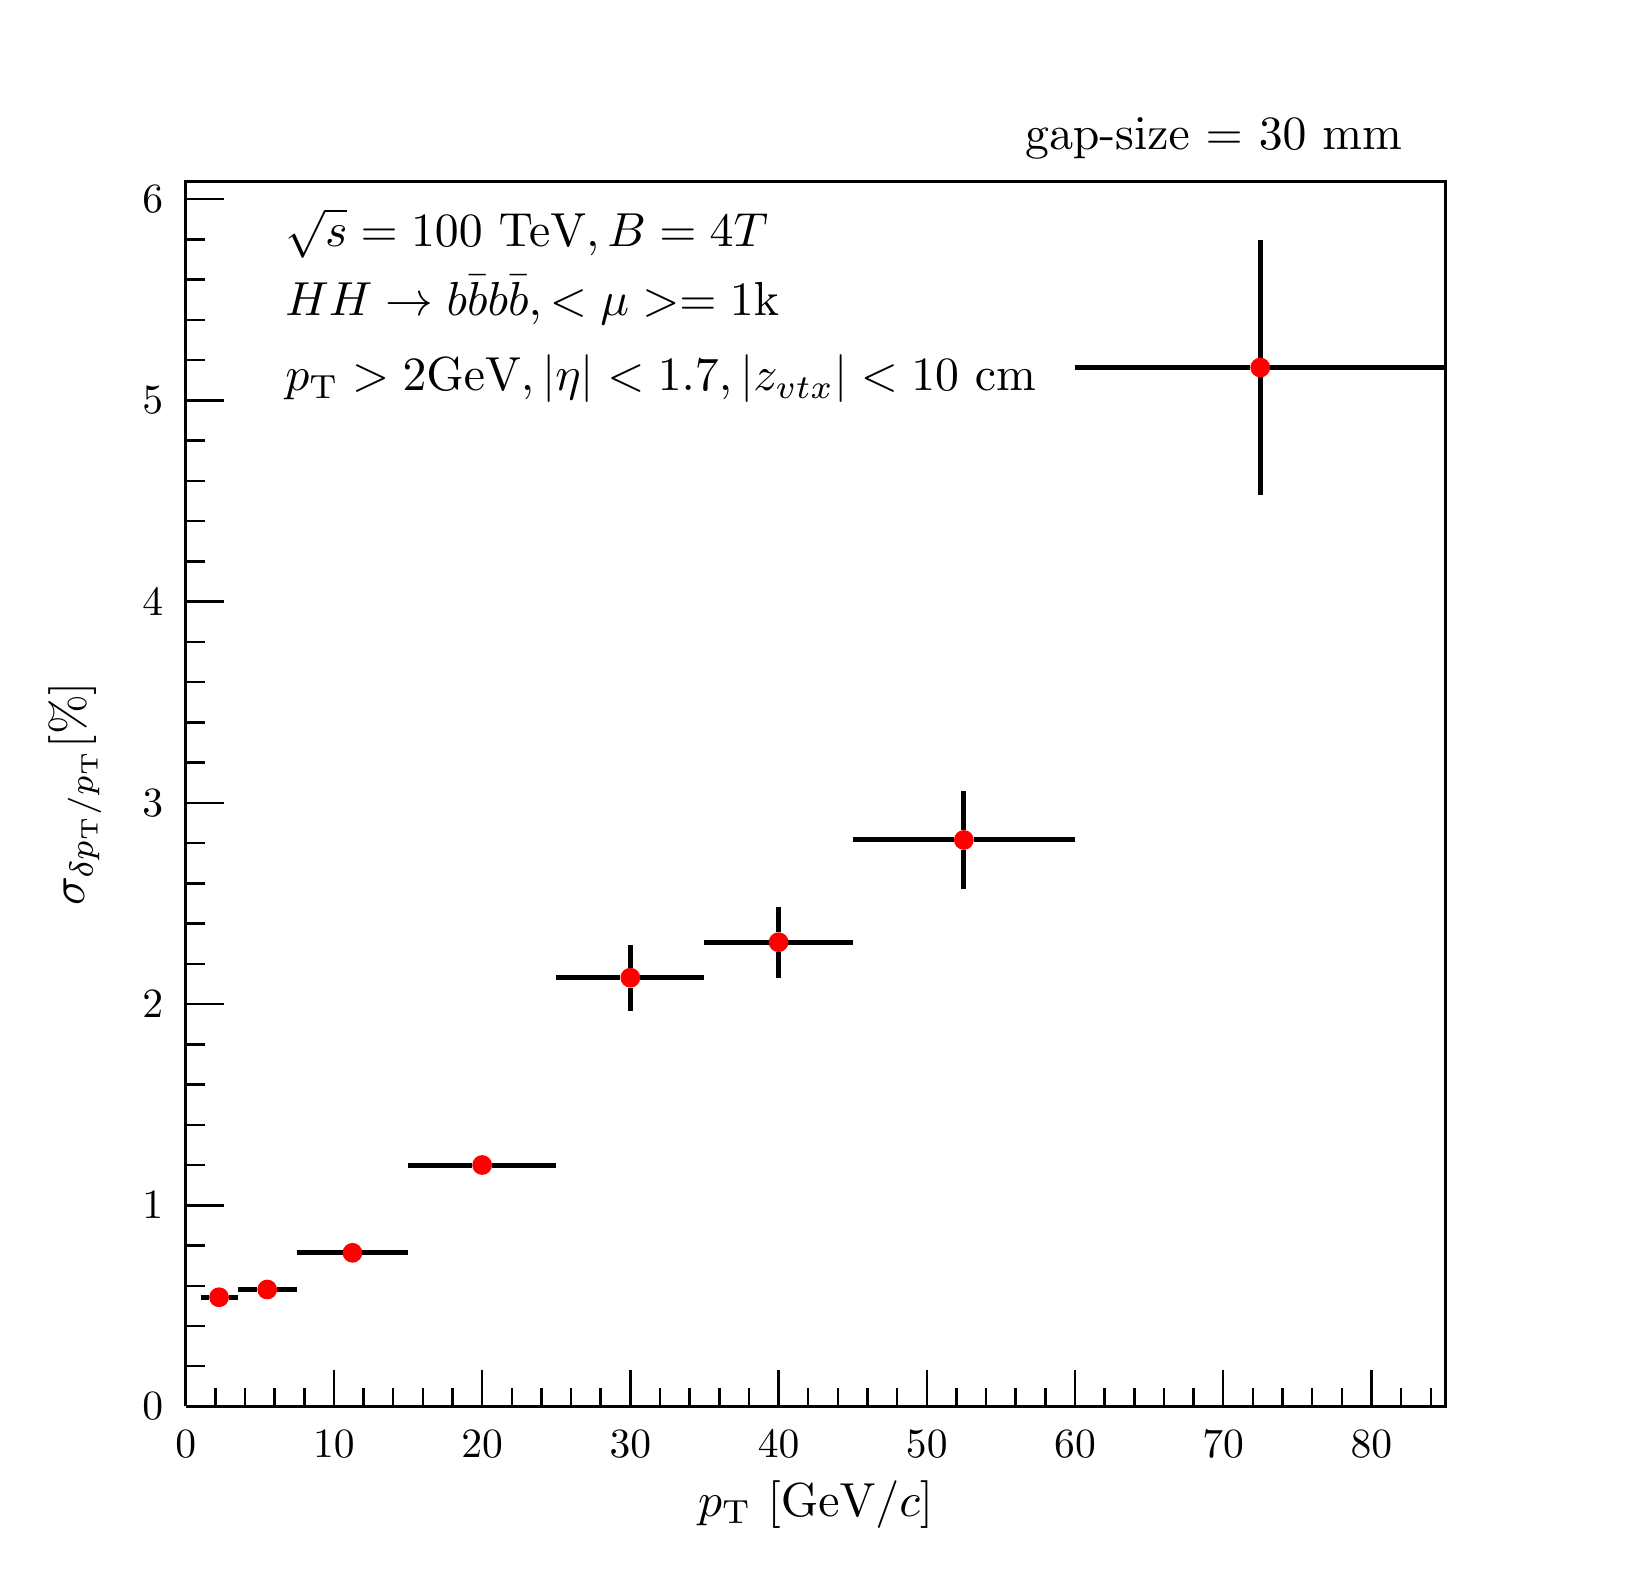
\begin{tikzpicture}
\pgfdeclareplotmark{cross} {
\pgfpathmoveto{\pgfpoint{-0.3\pgfplotmarksize}{\pgfplotmarksize}}
\pgfpathlineto{\pgfpoint{+0.3\pgfplotmarksize}{\pgfplotmarksize}}
\pgfpathlineto{\pgfpoint{+0.3\pgfplotmarksize}{0.3\pgfplotmarksize}}
\pgfpathlineto{\pgfpoint{+1\pgfplotmarksize}{0.3\pgfplotmarksize}}
\pgfpathlineto{\pgfpoint{+1\pgfplotmarksize}{-0.3\pgfplotmarksize}}
\pgfpathlineto{\pgfpoint{+0.3\pgfplotmarksize}{-0.3\pgfplotmarksize}}
\pgfpathlineto{\pgfpoint{+0.3\pgfplotmarksize}{-1.\pgfplotmarksize}}
\pgfpathlineto{\pgfpoint{-0.3\pgfplotmarksize}{-1.\pgfplotmarksize}}
\pgfpathlineto{\pgfpoint{-0.3\pgfplotmarksize}{-0.3\pgfplotmarksize}}
\pgfpathlineto{\pgfpoint{-1.\pgfplotmarksize}{-0.3\pgfplotmarksize}}
\pgfpathlineto{\pgfpoint{-1.\pgfplotmarksize}{0.3\pgfplotmarksize}}
\pgfpathlineto{\pgfpoint{-0.3\pgfplotmarksize}{0.3\pgfplotmarksize}}
\pgfpathclose
\pgfusepathqstroke
}
\pgfdeclareplotmark{cross*} {
\pgfpathmoveto{\pgfpoint{-0.3\pgfplotmarksize}{\pgfplotmarksize}}
\pgfpathlineto{\pgfpoint{+0.3\pgfplotmarksize}{\pgfplotmarksize}}
\pgfpathlineto{\pgfpoint{+0.3\pgfplotmarksize}{0.3\pgfplotmarksize}}
\pgfpathlineto{\pgfpoint{+1\pgfplotmarksize}{0.3\pgfplotmarksize}}
\pgfpathlineto{\pgfpoint{+1\pgfplotmarksize}{-0.3\pgfplotmarksize}}
\pgfpathlineto{\pgfpoint{+0.3\pgfplotmarksize}{-0.3\pgfplotmarksize}}
\pgfpathlineto{\pgfpoint{+0.3\pgfplotmarksize}{-1.\pgfplotmarksize}}
\pgfpathlineto{\pgfpoint{-0.3\pgfplotmarksize}{-1.\pgfplotmarksize}}
\pgfpathlineto{\pgfpoint{-0.3\pgfplotmarksize}{-0.3\pgfplotmarksize}}
\pgfpathlineto{\pgfpoint{-1.\pgfplotmarksize}{-0.3\pgfplotmarksize}}
\pgfpathlineto{\pgfpoint{-1.\pgfplotmarksize}{0.3\pgfplotmarksize}}
\pgfpathlineto{\pgfpoint{-0.3\pgfplotmarksize}{0.3\pgfplotmarksize}}
\pgfpathclose
\pgfusepathqfillstroke
}
\pgfdeclareplotmark{newstar} {
\pgfpathmoveto{\pgfqpoint{0pt}{\pgfplotmarksize}}
\pgfpathlineto{\pgfqpointpolar{44}{0.5\pgfplotmarksize}}
\pgfpathlineto{\pgfqpointpolar{18}{\pgfplotmarksize}}
\pgfpathlineto{\pgfqpointpolar{-20}{0.5\pgfplotmarksize}}
\pgfpathlineto{\pgfqpointpolar{-54}{\pgfplotmarksize}}
\pgfpathlineto{\pgfqpointpolar{-90}{0.5\pgfplotmarksize}}
\pgfpathlineto{\pgfqpointpolar{234}{\pgfplotmarksize}}
\pgfpathlineto{\pgfqpointpolar{198}{0.5\pgfplotmarksize}}
\pgfpathlineto{\pgfqpointpolar{162}{\pgfplotmarksize}}
\pgfpathlineto{\pgfqpointpolar{134}{0.5\pgfplotmarksize}}
\pgfpathclose
\pgfusepathqstroke
}
\pgfdeclareplotmark{newstar*} {
\pgfpathmoveto{\pgfqpoint{0pt}{\pgfplotmarksize}}
\pgfpathlineto{\pgfqpointpolar{44}{0.5\pgfplotmarksize}}
\pgfpathlineto{\pgfqpointpolar{18}{\pgfplotmarksize}}
\pgfpathlineto{\pgfqpointpolar{-20}{0.5\pgfplotmarksize}}
\pgfpathlineto{\pgfqpointpolar{-54}{\pgfplotmarksize}}
\pgfpathlineto{\pgfqpointpolar{-90}{0.5\pgfplotmarksize}}
\pgfpathlineto{\pgfqpointpolar{234}{\pgfplotmarksize}}
\pgfpathlineto{\pgfqpointpolar{198}{0.5\pgfplotmarksize}}
\pgfpathlineto{\pgfqpointpolar{162}{\pgfplotmarksize}}
\pgfpathlineto{\pgfqpointpolar{134}{0.5\pgfplotmarksize}}
\pgfpathclose
\pgfusepathqfillstroke
}
\definecolor{c}{rgb}{1,1,1};
\draw [color=c, fill=c] (0,0) rectangle (20,19.4486);
\draw [color=c, fill=c] (2,1.94486) rectangle (18,17.5038);
\definecolor{c}{rgb}{0,0,0};
\draw [c,line width=0.9] (2,1.94486) -- (2,17.5038) -- (18,17.5038) -- (18,1.94486) -- (2,1.94486);
\definecolor{c}{rgb}{1,1,1};
\draw [color=c, fill=c] (2,1.94486) rectangle (18,17.5038);
\definecolor{c}{rgb}{0,0,0};
\draw [c,line width=0.9] (2,1.94486) -- (2,17.5038) -- (18,17.5038) -- (18,1.94486) -- (2,1.94486);
\draw [c,line width=1.8] (2.18824,3.33184) -- (2.29822,3.33184);
\draw [c,line width=1.8] (2.54884,3.33184) -- (2.65882,3.33184);
\definecolor{c}{rgb}{1,0,0};
\foreach \P in {(2.42353,3.33184)}{\draw[mark options={color=c,fill=c},mark size=3.363363pt,mark=*] plot coordinates {\P};}
\definecolor{c}{rgb}{0,0,0};
\draw [c,line width=1.8] (2.65882,3.43023) -- (2.90998,3.43023);
\draw [c,line width=1.8] (3.16061,3.43023) -- (3.41176,3.43023);
\definecolor{c}{rgb}{1,0,0};
\foreach \P in {(3.03529,3.43023)}{\draw[mark options={color=c,fill=c},mark size=3.363363pt,mark=*] plot coordinates {\P};}
\definecolor{c}{rgb}{0,0,0};
\draw [c,line width=1.8] (3.41176,3.89651) -- (3.99233,3.89651);
\draw [c,line width=1.8] (4.24296,3.89651) -- (4.82353,3.89651);
\definecolor{c}{rgb}{1,0,0};
\foreach \P in {(4.11765,3.89651)}{\draw[mark options={color=c,fill=c},mark size=3.363363pt,mark=*] plot coordinates {\P};}
\definecolor{c}{rgb}{0,0,0};
\draw [c,line width=1.8] (4.82353,5.01113) -- (5.63939,5.01113);
\draw [c,line width=1.8] (5.89002,5.01113) -- (6.70588,5.01113);
\definecolor{c}{rgb}{1,0,0};
\foreach \P in {(5.76471,5.01113)}{\draw[mark options={color=c,fill=c},mark size=3.363363pt,mark=*] plot coordinates {\P};}
\definecolor{c}{rgb}{0,0,0};
\draw [c,line width=1.8] (7.64706,6.97075) -- (7.64706,7.26475);
\draw [c,line width=1.8] (7.64706,7.51538) -- (7.64706,7.80938);
\draw [c,line width=1.8] (6.70588,7.39006) -- (7.52175,7.39006);
\draw [c,line width=1.8] (7.77237,7.39006) -- (8.58823,7.39006);
\definecolor{c}{rgb}{1,0,0};
\foreach \P in {(7.64706,7.39006)}{\draw[mark options={color=c,fill=c},mark size=3.363363pt,mark=*] plot coordinates {\P};}
\definecolor{c}{rgb}{0,0,0};
\draw [c,line width=1.8] (9.52941,7.38987) -- (9.52941,7.71555);
\draw [c,line width=1.8] (9.52941,7.96618) -- (9.52941,8.29186);
\draw [c,line width=1.8] (8.58823,7.84087) -- (9.4041,7.84087);
\draw [c,line width=1.8] (9.65473,7.84087) -- (10.4706,7.84087);
\definecolor{c}{rgb}{1,0,0};
\foreach \P in {(9.52941,7.84087)}{\draw[mark options={color=c,fill=c},mark size=3.363363pt,mark=*] plot coordinates {\P};}
\definecolor{c}{rgb}{0,0,0};
\draw [c,line width=1.8] (11.8824,8.51593) -- (11.8824,9.01402);
\draw [c,line width=1.8] (11.8824,9.26465) -- (11.8824,9.76273);
\draw [c,line width=1.8] (10.4706,9.13933) -- (11.757,9.13933);
\draw [c,line width=1.8] (12.0077,9.13933) -- (13.2941,9.13933);
\definecolor{c}{rgb}{1,0,0};
\foreach \P in {(11.8824,9.13933)}{\draw[mark options={color=c,fill=c},mark size=3.363363pt,mark=*] plot coordinates {\P};}
\definecolor{c}{rgb}{0,0,0};
\draw [c,line width=1.8] (15.6471,13.5153) -- (15.6471,15.0138);
\draw [c,line width=1.8] (15.6471,15.2644) -- (15.6471,16.7629);
\draw [c,line width=1.8] (13.2941,15.1391) -- (15.5217,15.1391);
\draw [c,line width=1.8] (15.7724,15.1391) -- (18,15.1391);
\definecolor{c}{rgb}{1,0,0};
\foreach \P in {(15.6471,15.1391)}{\draw[mark options={color=c,fill=c},mark size=3.363363pt,mark=*] plot coordinates {\P};}
\definecolor{c}{rgb}{0,0,0};
\draw [c,line width=0.9] (2,1.94486) -- (18,1.94486);
\draw [c,line width=0.9] (2,2.41163) -- (2,1.94486);
\draw [c,line width=0.9] (2.37647,2.17825) -- (2.37647,1.94486);
\draw [c,line width=0.9] (2.75294,2.17825) -- (2.75294,1.94486);
\draw [c,line width=0.9] (3.12941,2.17825) -- (3.12941,1.94486);
\draw [c,line width=0.9] (3.50588,2.17825) -- (3.50588,1.94486);
\draw [c,line width=0.9] (3.88235,2.41163) -- (3.88235,1.94486);
\draw [c,line width=0.9] (4.25882,2.17825) -- (4.25882,1.94486);
\draw [c,line width=0.9] (4.63529,2.17825) -- (4.63529,1.94486);
\draw [c,line width=0.9] (5.01177,2.17825) -- (5.01177,1.94486);
\draw [c,line width=0.9] (5.38824,2.17825) -- (5.38824,1.94486);
\draw [c,line width=0.9] (5.76471,2.41163) -- (5.76471,1.94486);
\draw [c,line width=0.9] (6.14118,2.17825) -- (6.14118,1.94486);
\draw [c,line width=0.9] (6.51765,2.17825) -- (6.51765,1.94486);
\draw [c,line width=0.9] (6.89412,2.17825) -- (6.89412,1.94486);
\draw [c,line width=0.9] (7.27059,2.17825) -- (7.27059,1.94486);
\draw [c,line width=0.9] (7.64706,2.41163) -- (7.64706,1.94486);
\draw [c,line width=0.9] (8.02353,2.17825) -- (8.02353,1.94486);
\draw [c,line width=0.9] (8.4,2.17825) -- (8.4,1.94486);
\draw [c,line width=0.9] (8.77647,2.17825) -- (8.77647,1.94486);
\draw [c,line width=0.9] (9.15294,2.17825) -- (9.15294,1.94486);
\draw [c,line width=0.9] (9.52941,2.41163) -- (9.52941,1.94486);
\draw [c,line width=0.9] (9.90588,2.17825) -- (9.90588,1.94486);
\draw [c,line width=0.9] (10.2824,2.17825) -- (10.2824,1.94486);
\draw [c,line width=0.9] (10.6588,2.17825) -- (10.6588,1.94486);
\draw [c,line width=0.9] (11.0353,2.17825) -- (11.0353,1.94486);
\draw [c,line width=0.9] (11.4118,2.41163) -- (11.4118,1.94486);
\draw [c,line width=0.9] (11.7882,2.17825) -- (11.7882,1.94486);
\draw [c,line width=0.9] (12.1647,2.17825) -- (12.1647,1.94486);
\draw [c,line width=0.9] (12.5412,2.17825) -- (12.5412,1.94486);
\draw [c,line width=0.9] (12.9176,2.17825) -- (12.9176,1.94486);
\draw [c,line width=0.9] (13.2941,2.41163) -- (13.2941,1.94486);
\draw [c,line width=0.9] (13.6706,2.17825) -- (13.6706,1.94486);
\draw [c,line width=0.9] (14.0471,2.17825) -- (14.0471,1.94486);
\draw [c,line width=0.9] (14.4235,2.17825) -- (14.4235,1.94486);
\draw [c,line width=0.9] (14.8,2.17825) -- (14.8,1.94486);
\draw [c,line width=0.9] (15.1765,2.41163) -- (15.1765,1.94486);
\draw [c,line width=0.9] (15.5529,2.17825) -- (15.5529,1.94486);
\draw [c,line width=0.9] (15.9294,2.17825) -- (15.9294,1.94486);
\draw [c,line width=0.9] (16.3059,2.17825) -- (16.3059,1.94486);
\draw [c,line width=0.9] (16.6824,2.17825) -- (16.6824,1.94486);
\draw [c,line width=0.9] (17.0588,2.41163) -- (17.0588,1.94486);
\draw [c,line width=0.9] (17.0588,2.41163) -- (17.0588,1.94486);
\draw [c,line width=0.9] (17.4353,2.17825) -- (17.4353,1.94486);
\draw [c,line width=0.9] (17.8118,2.17825) -- (17.8118,1.94486);
\draw [anchor=base] (2,1.30306) node[scale=1.50291, color=c, rotate=0]{0};
\draw [anchor=base] (3.88235,1.30306) node[scale=1.50291, color=c, rotate=0]{10};
\draw [anchor=base] (5.76471,1.30306) node[scale=1.50291, color=c, rotate=0]{20};
\draw [anchor=base] (7.64706,1.30306) node[scale=1.50291, color=c, rotate=0]{30};
\draw [anchor=base] (9.52941,1.30306) node[scale=1.50291, color=c, rotate=0]{40};
\draw [anchor=base] (11.4118,1.30306) node[scale=1.50291, color=c, rotate=0]{50};
\draw [anchor=base] (13.2941,1.30306) node[scale=1.50291, color=c, rotate=0]{60};
\draw [anchor=base] (15.1765,1.30306) node[scale=1.50291, color=c, rotate=0]{70};
\draw [anchor=base] (17.0588,1.30306) node[scale=1.50291, color=c, rotate=0]{80};
\draw (10,0.700151) node[scale=1.72557, color=c, rotate=0]{$p_{\text{T}} ~[\text{GeV}/c]$};
\draw [c,line width=0.9] (2,1.94486) -- (2,17.5038);
\draw [c,line width=0.9] (2.48,1.94486) -- (2,1.94486);
\draw [c,line width=0.9] (2.24,2.45592) -- (2,2.45592);
\draw [c,line width=0.9] (2.24,2.96698) -- (2,2.96698);
\draw [c,line width=0.9] (2.24,3.47804) -- (2,3.47804);
\draw [c,line width=0.9] (2.24,3.9891) -- (2,3.9891);
\draw [c,line width=0.9] (2.48,4.50016) -- (2,4.50016);
\draw [c,line width=0.9] (2.24,5.01122) -- (2,5.01122);
\draw [c,line width=0.9] (2.24,5.52227) -- (2,5.52227);
\draw [c,line width=0.9] (2.24,6.03333) -- (2,6.03333);
\draw [c,line width=0.9] (2.24,6.54439) -- (2,6.54439);
\draw [c,line width=0.9] (2.48,7.05545) -- (2,7.05545);
\draw [c,line width=0.9] (2.24,7.56651) -- (2,7.56651);
\draw [c,line width=0.9] (2.24,8.07757) -- (2,8.07757);
\draw [c,line width=0.9] (2.24,8.58863) -- (2,8.58863);
\draw [c,line width=0.9] (2.24,9.09969) -- (2,9.09969);
\draw [c,line width=0.9] (2.48,9.61074) -- (2,9.61074);
\draw [c,line width=0.9] (2.24,10.1218) -- (2,10.1218);
\draw [c,line width=0.9] (2.24,10.6329) -- (2,10.6329);
\draw [c,line width=0.9] (2.24,11.1439) -- (2,11.1439);
\draw [c,line width=0.9] (2.24,11.655) -- (2,11.655);
\draw [c,line width=0.9] (2.48,12.166) -- (2,12.166);
\draw [c,line width=0.9] (2.24,12.6771) -- (2,12.6771);
\draw [c,line width=0.9] (2.24,13.1882) -- (2,13.1882);
\draw [c,line width=0.9] (2.24,13.6992) -- (2,13.6992);
\draw [c,line width=0.9] (2.24,14.2103) -- (2,14.2103);
\draw [c,line width=0.9] (2.48,14.7213) -- (2,14.7213);
\draw [c,line width=0.9] (2.24,15.2324) -- (2,15.2324);
\draw [c,line width=0.9] (2.24,15.7434) -- (2,15.7434);
\draw [c,line width=0.9] (2.24,16.2545) -- (2,16.2545);
\draw [c,line width=0.9] (2.24,16.7656) -- (2,16.7656);
\draw [c,line width=0.9] (2.48,17.2766) -- (2,17.2766);
\draw [c,line width=0.9] (2.48,17.2766) -- (2,17.2766);
\draw [anchor= east] (1.9,1.94486) node[scale=1.50291, color=c, rotate=0]{0};
\draw [anchor= east] (1.9,4.50016) node[scale=1.50291, color=c, rotate=0]{1};
\draw [anchor= east] (1.9,7.05545) node[scale=1.50291, color=c, rotate=0]{2};
\draw [anchor= east] (1.9,9.61074) node[scale=1.50291, color=c, rotate=0]{3};
\draw [anchor= east] (1.9,12.166) node[scale=1.50291, color=c, rotate=0]{4};
\draw [anchor= east] (1.9,14.7213) node[scale=1.50291, color=c, rotate=0]{5};
\draw [anchor= east] (1.9,17.2766) node[scale=1.50291, color=c, rotate=0]{6};
\draw (0.592,9.72431) node[scale=1.72557, color=c, rotate=90]{$\sigma_{\delta p_{\text{T}}/p_{\text{T}}} [\%]$};
\draw [anchor=base west] (3.05,16.6748) node[scale=1.72557, color=c, rotate=0]{$\sqrt{s} = 100 ~\text{TeV}, B = 4T$};
\draw [anchor=base west] (3.05,15.7996) node[scale=1.72557, color=c, rotate=0]{$HH \rightarrow b\bar{b}b\bar{b}, <\mu> = \text{1k}$};
\draw [anchor=base west] (3.05,14.8432) node[scale=1.72557, color=c, rotate=0]{$p_{\text{T}} > 2\text{GeV}, |\eta| < 1.7, |z_{vtx}| < 10\text{~cm}$};
\draw [anchor=base west] (12.445,17.9122) node[scale=1.72557, color=c, rotate=0]{gap-size = 30 mm};
\draw [anchor=base west] (12.445,17.5232) node[scale=1.72557, color=c, rotate=0]{ };
\end{tikzpicture}
% end document
\end{document}
